\subsection{Historias de Usuarios}

Las HU son la técnica que utiliza XP para especificar los requisitos de software, estas deben ser programadas en un tiempo entre una y tres semanas. Si la estimación es superior a las tres semanas, debe ser dividida en dos o más historias. Si es menos de una semana, se debe combinar con otra HU. Las estimaciones de esfuerzo, asociado a la implementación de las historias, la establecen los programadores, utilizando como medida el punto. Un punto, equivale a una semana ideal de programación (5 días laborables). Las historias, generalmente, valen de 1 a 3 puntos. \citep{escribano2002introduccion}. A continuación se describen las HU definidas parra llevar a cabo el desarrollo de los módulos.


\begin{userstory}[tb:prueba]
	\storyname{Registro de Usuario}
	\storyuser{Administrador, Usuario}
	\storyiter{1}
	\storypriority{Alta}
	\storyrisk{Bajo}
	\storypoints{2}
	\storyprogrammer{Técn. Carlos Brayan Rámila Chorens}
	\storydescription{
		Como usuario nuevo, quiero poder registrarme en la aplicación proporcionando mi información personal, como nombre, dirección de correo electrónico y contraseña, para acceder a las funcionalidades de la aplicación.
		\begin{itemize}
			\item nombre
			\item dirección de correo electrónico
			\item contraseña
			\item carnet de identidad
		\end{itemize}
	}
	\storyobservation{
		\begin{itemize}
			\item La aplicación debe permitir al usuario completar un formulario de registro con campos para nombre, correo electrónico y contraseña.
			\item Los campos del formulario deben validar que la información ingresada sea válida y esté en el formato correcto.
			\item Después de enviar el formulario, la aplicación debe crear una cuenta de usuario y almacenarla en la base de datos.
			\item Se debe enviar un correo electrónico de confirmación al usuario registrado para verificar su dirección de correo electrónico.
			\item El usuario debe poder iniciar sesión después de completar el registro exitosamente.
		\end{itemize}
	}
	%\storyinterface{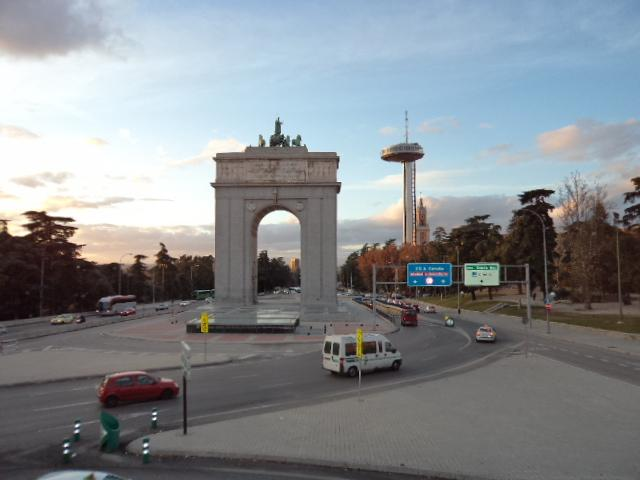
\includegraphics[scale=0.5]{Images/DSC00461}}
\end{userstory}


\begin{userstory}[tb:prueba]
	\storyname{Iniciar Sesión}
	\storyuser{Administrador, Usuario}
	\storyiter{1}
	\storypriority{Alta}
	\storyrisk{Bajo}
	\storypoints{2}
	\storyprogrammer{Técn. Carlos Brayan Rámila Chorens}
	\storydescription{
		Como usuario registrado, quiero poder iniciar sesión en la aplicación utilizando mi dirección de correo electrónico y contraseña, para acceder a mis datos y realizar acciones dentro de la aplicación.
		\begin{itemize}
			\item dirección de correo electrónico
			\item contraseña
		\end{itemize}
	}	
	\storyobservation{
		\begin{itemize}
			\item La aplicación debe proporcionar un formulario de inicio de sesión con campos para correo electrónico y contraseña.
			\item Los campos del formulario deben validar que la información ingresada sea válida y coincida con los datos almacenados en la base de datos.
			\item Después de enviar el formulario, la aplicación debe autenticar al usuario y redirigirlo a la página principal si las credenciales son válidas.
			\item Si las credenciales son inválidas, la aplicación debe mostrar un mensaje de error al usuario indicando que las credenciales son incorrectas.
			\item La sesión del usuario debe mantenerse activa mientras navega por la aplicación, permitiéndole acceder a las funcionalidades protegidas sin necesidad de volver a iniciar sesión.
		\end{itemize}
	}
	%\storyinterface{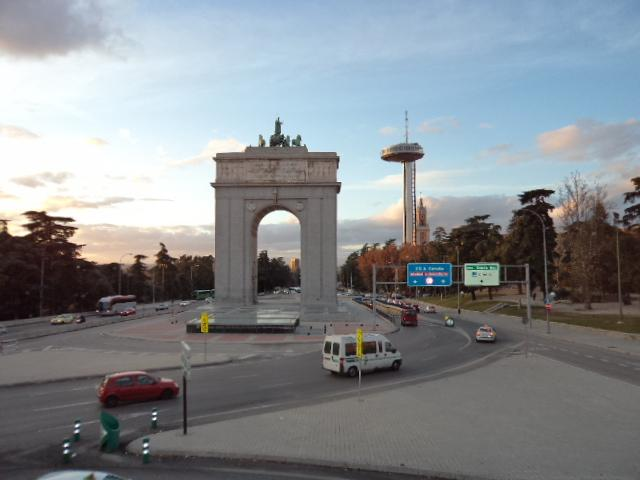
\includegraphics[scale=0.5]{Images/DSC00461}}
\end{userstory}


\begin{userstory}[tb:prueba]
	\storyname{Gestión de Perfiles de Usuario}
	\storyuser{Administrador}
	\storyiter{1}
	\storypriority{Alta}
	\storyrisk{Bajo}
	\storypoints{1}
	\storyprogrammer{Técn. Carlos Brayan Rámila Chorens}
	\storydescription{
		Como administrador, quiero poder gestionar los perfiles de usuario, incluyendo la capacidad de crear, editar y eliminar cuentas de usuario, para mantener el control sobre quién tiene acceso a la aplicación.
		\begin{itemize}
			\item nombre
			\item dirección de correo electrónico
			\item contraseña
			\item carnet de identidad
		\end{itemize}
	}	
	\storyobservation{
		\begin{itemize}
			\item La aplicación debe proporcionar una interfaz de administración donde el administrador pueda ver una lista de todos los usuarios registrados.
			\item El administrador debe poder crear nuevos perfiles de usuario, proporcionando información como nombre, dirección de correo electrónico y contraseña.
			\item Se debe implementar la funcionalidad de edición para permitir al administrador actualizar la información de los perfiles de usuario existentes.
			\item El administrador debe poder eliminar cuentas de usuario cuando sea necesario, lo que resultará en la eliminación permanente de los datos asociados con esa cuenta.
			\item Se deben implementar controles de acceso adecuados para garantizar que solo el administrador tenga acceso a estas funcionalidades de gestión de perfiles.
		\end{itemize}
	}
	%\storyinterface{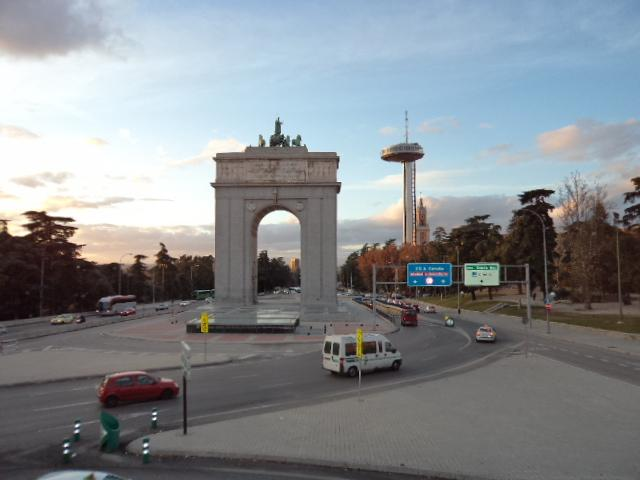
\includegraphics[scale=0.5]{Images/DSC00461}}
\end{userstory}

\begin{userstory}[tb:prueba]
	\storyname{Registrar Cita}
	\storyuser{Cliente}
	\storyiter{1.5}
	\storypriority{Alta}
	\storyrisk{Media}
	\storypoints{2}
	\storyprogrammer{Técn. Carlos Brayan Rámila Chorens}
	\storydescription{
		Permite al usuario poder acceder a la opción de registrar su cita, donde se muestra una página con un formulario a rellenar con los siguientes campos
		\begin{itemize}
			\item Nombre
			\item Apellidos
			\item Usuario
			\item Contraseña
			\item Dirección Particular
			\item Ci
			\item Teléfono de localización 
			\item Cantidad de Documentos a Legalizar
			\item Obtención de documentos
		\end{itemize}
	}	
	\storyobservation{
	}
	%\storyinterface{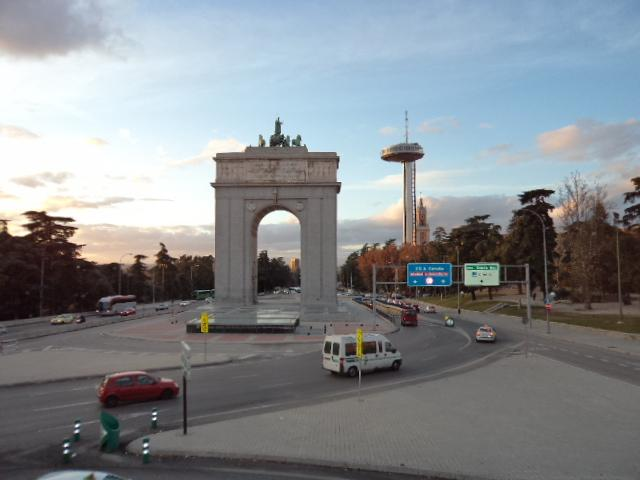
\includegraphics[scale=0.5]{Images/DSC00461}}
\end{userstory}

\begin{userstory}[tb:prueba]
	\storyname{Autenticar Usuario}
	\storyuser{Administrador, Legalizador, Cliente, Registradora, Notario}
	\storyiter{1}
	\storypriority{Alta}
	\storyrisk{Media}
	\storypoints{2}
	\storyprogrammer{Técn. Carlos Brayan Rámila Chorens}
	\storydescription{
		Permite al usuario poder acceder a la opción de autenticarse en el sistema, donde se muestra una la página principal mediante estos campos.
		\begin{itemize}
			\item Usuario 
			\item Contraseña
		\end{itemize}
	}	
	\storyobservation{
	}
	%\storyinterface{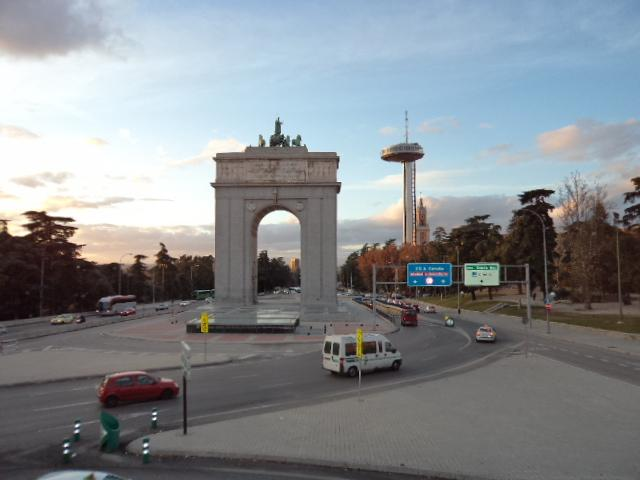
\includegraphics[scale=0.5]{Images/DSC00461}}
\end{userstory}

\begin{userstory}[tb:prueba]
	\storyname{Modificar Usuario}
	\storyuser{Administrador}
	\storyiter{1}
	\storypriority{Alta}
	\storyrisk{Media}
	\storypoints{2}
	\storyprogrammer{Técn. Carlos Brayan Rámila Chorens}
	\storydescription{
		Permite al usuario poder acceder a la opción de modificar usuario, donde se muestra una página con un formulario con los datos que el usuario puede modificar los cuales son.
		\begin{itemize}
			\item Nombre
			\item Apellidos
			\item Usuario
			
		\end{itemize}
	}	
	\storyobservation{
	}
	%\storyinterface{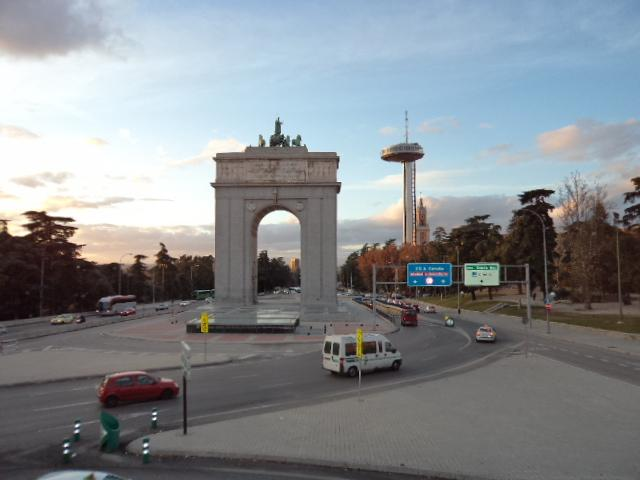
\includegraphics[scale=0.5]{Images/DSC00461}}
\end{userstory}

\begin{userstory}[tb:prueba]
	\storyname{Registrar Usuario}
	\storyuser{Administrador}
	\storyiter{1}
	\storypriority{Alta}
	\storyrisk{Media}
	\storypoints{2}
	\storyprogrammer{Técn. Carlos Brayan Rámila Chorens}
	\storydescription{
		Permite al usuario poder acceder a la opción de registrar usuario, donde se muestra una página con un formulario a rellenar con los siguientes datos.
		\begin{itemize}
			\item Nombre
			\item Apellidos
			\item Contraseña
			\item Usuario
		\end{itemize}
	}	
	\storyobservation{
	}
	%\storyinterface{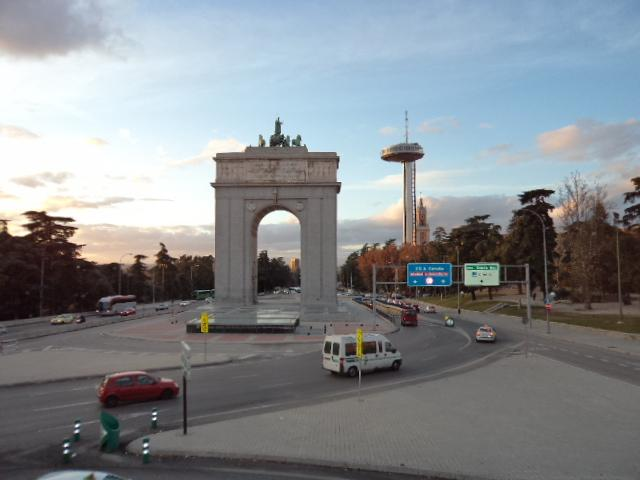
\includegraphics[scale=0.5]{Images/DSC00461}}
\end{userstory}

\begin{userstory}[tb:prueba]
	\storyname{Eliminar Usuario}
	\storyuser{Administrador}
	\storyiter{1}
	\storypriority{Alta}
	\storyrisk{Media}
	\storypoints{2}
	\storyprogrammer{Técn. Carlos Brayan Rámila Chorens}
	\storydescription{
		Permite al usuario poder acceder a la opción de eliminar usuario, donde se muestra una página con un mensaje de advertencia.
		Estas seguro
		¡No podrás revertir esto!
	}
	\storyobservation{
	}	
	%\storyinterface{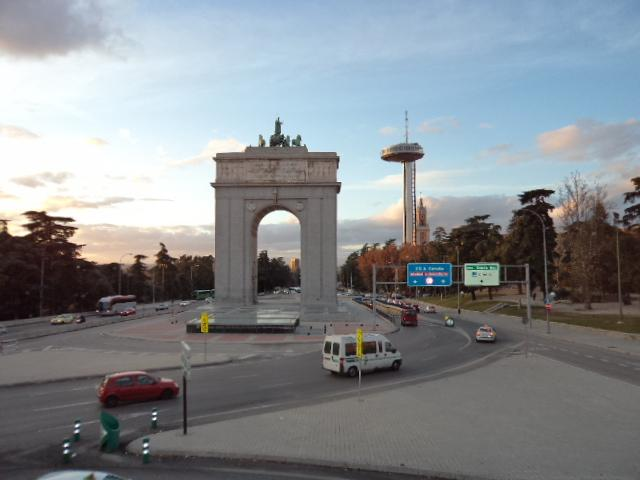
\includegraphics[scale=0.5]{Images/DSC00461}}
\end{userstory}

% Notificar via SMS
\begin{userstory}[tb:prueba]
	\storyname{Notificar via SMS}
	\storyuser{Cliente}
	\storyiter{1.5}
	\storypriority{Alta}
	\storyrisk{Media}
	\storypoints{2}
	\storyprogrammer{Técn. Carlos Brayan Rámila Chorens}
	\storydescription{
		Permite al usuario recibir una notificación a su teléfono móvil, sobre que la cita ha sido realizada de forma exitosa. Mostrando el siguiente texto.
		Su cita ha sido programada para (fecha del dia de la cita) y lugar (dirección de la entidad)
	}
	\storyobservation{
	}	
	%\storyinterface{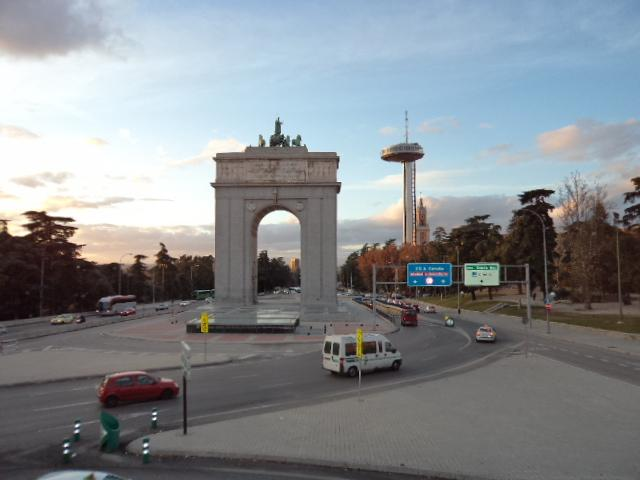
\includegraphics[scale=0.5]{Images/DSC00461}}
\end{userstory}

% Crear Contrato
\begin{userstory}[tb:prueba]
	\storyname{Crear Contrato}
	\storyuser{Registradora}
	\storyiter{1.5}
	\storypriority{Alta}
	\storyrisk{Media}
	\storypoints{2}
	\storyprogrammer{Técn. Carlos Brayan Rámila Chorens}
	\storydescription{
		Descripción:
		Permite al usuario poder acceder a la opción de crear contrato, donde se muestra una página con el contrato previamente elaborado, mostrando los siguientes datos.
		
		\begin{itemize}
			\item Datos generales del cliente (nombre y apellidos, ci)
			\item Residente (dirección particular)
			\item Teléfono de localización 
			\item Beneficiario (nombre y apellidos)
			\item Tipo y Cantidad de Documentos 
			\item Codigo 
			\item Sellos
			\item Nombre y apellidos de la legalizadora que realiza el contrato 
			\item Valor total del contrato
			\item Valor de los sellos
		\end{itemize}
		
	}
	\storyobservation{
	}	
	%\storyinterface{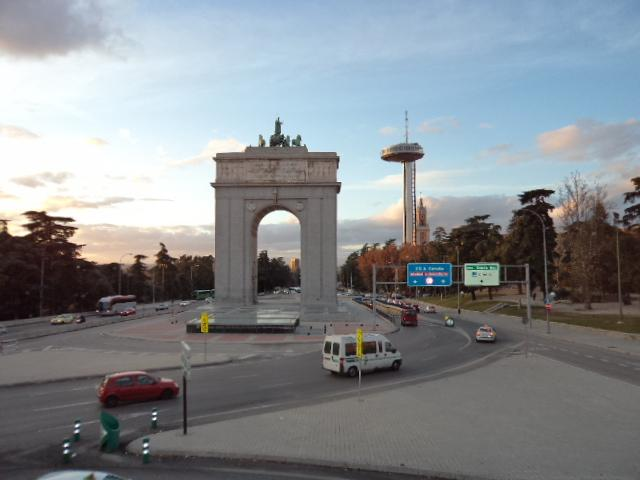
\includegraphics[scale=0.5]{Images/DSC00461}}
\end{userstory}

% Modificar Contrato
\begin{userstory}[tb:prueba]
	\storyname{Modificar Contrato}
	\storyuser{Registradora}
	\storyiter{1.5}
	\storypriority{Alta}
	\storyrisk{Media}
	\storypoints{2}
	\storyprogrammer{Técn. Carlos Brayan Rámila Chorens}
	\storydescription{
		Permite al usuario poder acceder a la opción de modificar contrato, donde se muestra una página con el contrato previamente elaborado, mostrando los siguientes datos.
				
		\begin{itemize}
			\item Datos generales del cliente (nombre y apellidos, ci)
			\item Residente (dirección particular)
			\item Teléfono de localización 
			\item Beneficiario (nombre y apellidos)
			\item Tipo y Cantidad de Documentos 
			\item Codigo 
			\item Sellos
			\item Nombre y apellidos de la legalizadora que realiza el contrato 
			\item Valor total del contrato
			\item Valor de los sellos
		\end{itemize}
		
	}	
	\storyobservation{
	}
	%\storyinterface{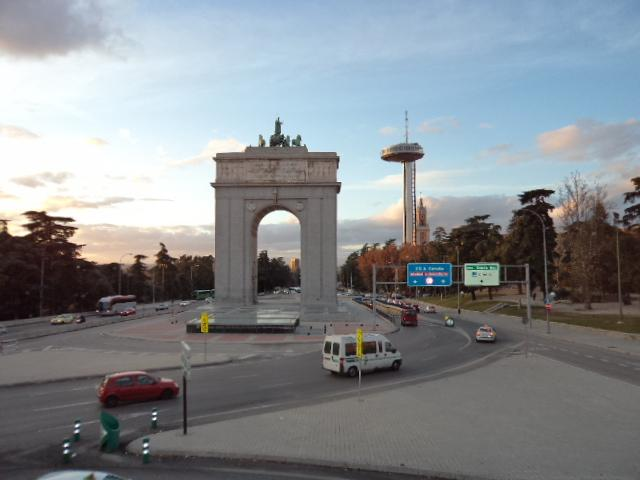
\includegraphics[scale=0.5]{Images/DSC00461}}
\end{userstory}

% Eliminar Contrato
\begin{userstory}[tb:prueba]
	\storyname{Eliminar Contrato}
	\storyuser{Legalizador}
	\storyiter{1.5}
	\storypriority{Alta}
	\storyrisk{Media}
	\storypoints{2}
	\storyprogrammer{Técn. Carlos Brayan Rámila Chorens}
	\storydescription{
		Permite al usuario poder acceder a la opción de eliminar contrato, donde se muestra una página con un mensaje de advertencia.
		Estas seguro
		¡No podrás revertir esto!

	}
	\storyobservation{
	}	
	%\storyinterface{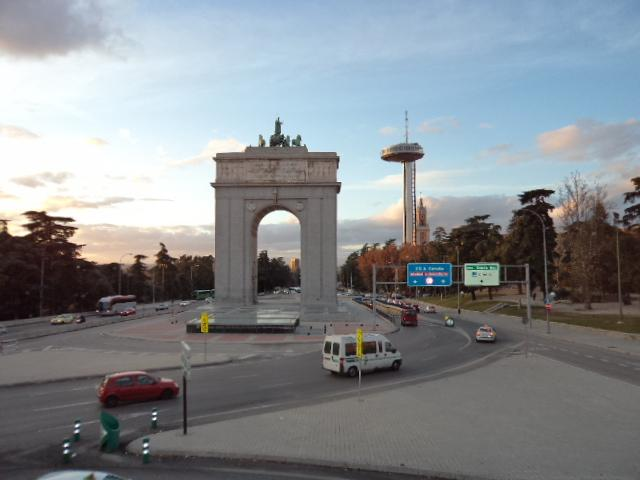
\includegraphics[scale=0.5]{Images/DSC00461}}
\end{userstory}

% Imprimir Contrato
\begin{userstory}[tb:prueba]
	\storyname{Imprimir Contrato}
	\storyuser{Legalizador}
	\storyiter{4}
	\storypriority{Alta}
	\storyrisk{Media}
	\storypoints{2}
	\storyprogrammer{Técn. Carlos Brayan Rámila Chorens}
	\storydescription{
		Permite al usuario poder acceder a la opción de imprimir contrato 2 copias.
		
	}	
	\storyobservation{
	}
	%\storyinterface{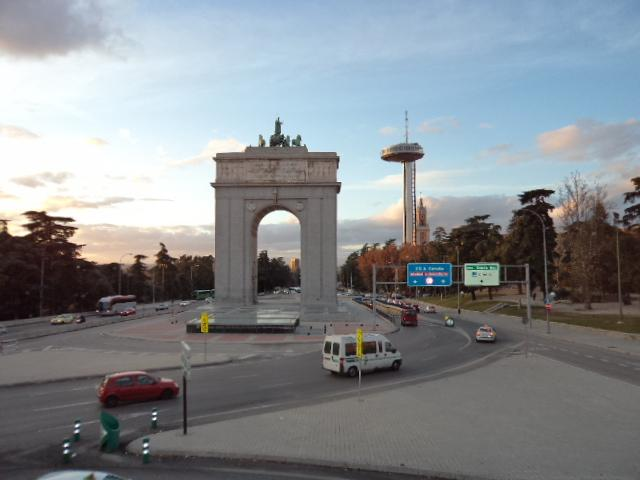
\includegraphics[scale=0.5]{Images/DSC00461}}
\end{userstory}

% Crear Tramite
\begin{userstory}[tb:prueba]
	\storyname{Crear Tramite}
	\storyuser{Administrador}
	\storyiter{4}
	\storypriority{Alta}
	\storyrisk{Media}
	\storypoints{2}
	\storyprogrammer{Técn. Carlos Brayan Rámila Chorens}
	\storydescription{
		Permite al usuario poder acceder a la opción de crear un trámite a realizar, donde se muestra una página con un formulario a rellenar con los siguientes datos:
			
		\begin{itemize}
			\item Codigo
			\item Descripcion
			\item Precio
		\end{itemize}
		
		
	}
	\storyobservation{
	}	
	%\storyinterface{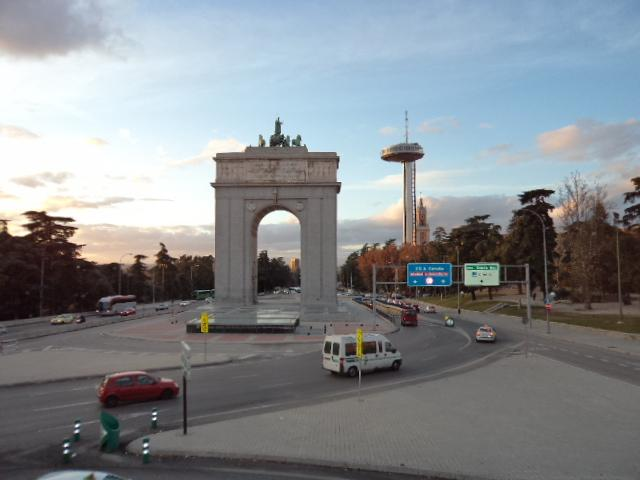
\includegraphics[scale=0.5]{Images/DSC00461}}
\end{userstory}

% Modificar  Tramite
\begin{userstory}[tb:prueba]
	\storyname{Modificar  Tramite}
	\storyuser{Administrador}
	\storyiter{4}
	\storypriority{Alta}
	\storyrisk{Media}
	\storypoints{2}
	\storyprogrammer{Técn. Carlos Brayan Rámila Chorens}
	\storydescription{
		Permite al usuario poder acceder a la opción de modificar un trámite a realizar, donde se muestra una página con un formulario con los siguientes datos:
		
		\begin{itemize}
			\item Codigo
			\item Descripcion
			\item Precio
		\end{itemize}
		
		
	}	
	\storyobservation{
	}
	%\storyinterface{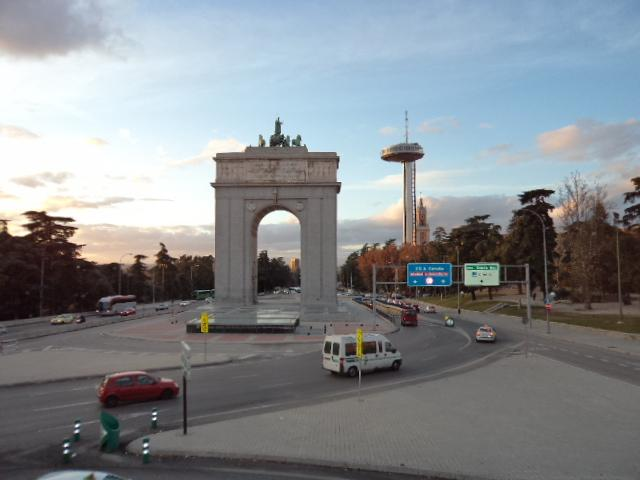
\includegraphics[scale=0.5]{Images/DSC00461}}
\end{userstory}

% Eliminar Tramite
\begin{userstory}[tb:prueba]
	\storyname{Eliminar   Tramite}
	\storyuser{Administrador}
	\storyiter{4}
	\storypriority{Alta}
	\storyrisk{Media}
	\storypoints{2}
	\storyprogrammer{Técn. Carlos Brayan Rámila Chorens}
	\storydescription{
		Permite al usuario poder acceder a la opción de eliminar , donde se muestra una página con un mensaje de advertencia.
		Estas seguro
		¡No podrás revertir esto!		
		
	}	
	\storyobservation{
	}
	%\storyinterface{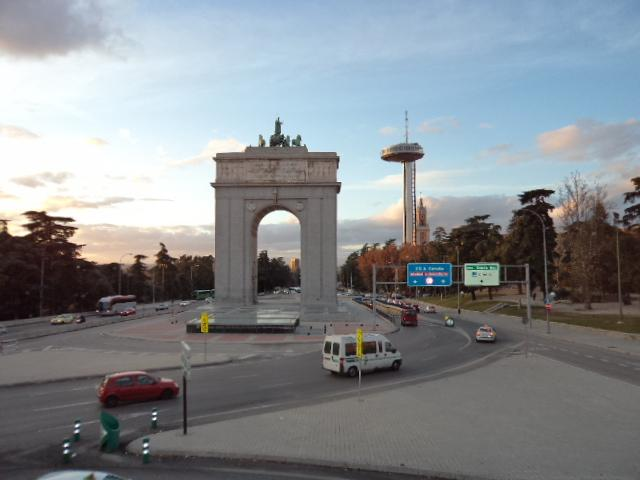
\includegraphics[scale=0.5]{Images/DSC00461}}
\end{userstory}

% Crear Prefactura
\begin{userstory}[tb:prueba]
	\storyname{Crear Prefactura}
	\storyuser{Legalizador}
	\storyiter{4}
	\storypriority{Alta}
	\storyrisk{Media}
	\storypoints{2}
	\storyprogrammer{Técn. Carlos Brayan Rámila Chorens}
	\storydescription{
		Permite al usuario poder acceder a la opción de crear una prefactura realizar, donde se muestra una página con un formulario a rellenar con los siguientes datos:
		
		\begin{itemize}
			\item Codigo
			\item Nombre
			\item Orden de Trabajo
			\item No
			\item Fecha
			\item Direccion
		\end{itemize}
		

	}	
	\storyobservation{
	}
	%\storyinterface{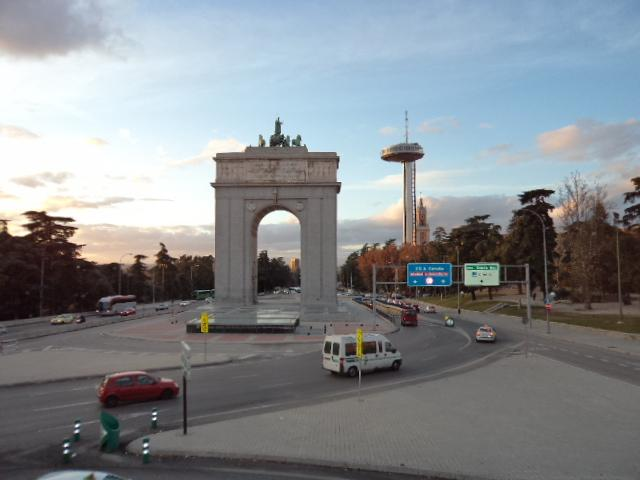
\includegraphics[scale=0.5]{Images/DSC00461}}
\end{userstory}

% Modificar Prefactura
\begin{userstory}[tb:prueba]
	\storyname{Modificar Prefactura}
	\storyuser{Legalizador}
	\storyiter{4}
	\storypriority{Alta}
	\storyrisk{Media}
	\storypoints{2}
	\storyprogrammer{Técn. Carlos Brayan Rámila Chorens}
	\storydescription{
		Permite al usuario poder acceder a la opción de modificar un trámite a realizar, donde se muestra una página con un formulario con los siguientes datos:
		
		\begin{itemize}
			\item Codigo
			\item Nombre
			\item Orden de Trabajo
			\item No
			\item Fecha
			\item Direccion
		\end{itemize}
		
	}	
	\storyobservation{
	}
	%\storyinterface{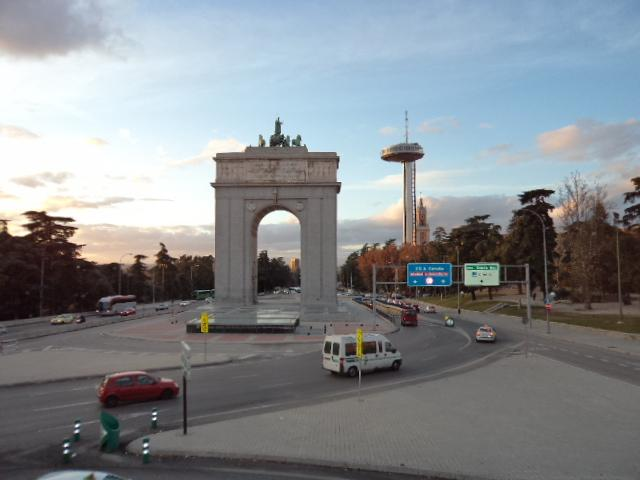
\includegraphics[scale=0.5]{Images/DSC00461}}
\end{userstory}

% Eliminar Prefactura
\begin{userstory}[tb:prueba]
	\storyname{Eliminar Prefactura}
	\storyuser{Legalizador}
	\storyiter{4}
	\storypriority{Alta}
	\storyrisk{Media}
	\storypoints{2}
	\storyprogrammer{Técn. Carlos Brayan Rámila Chorens}
	\storydescription{
			Permite al usuario poder acceder a la opción de eliminar Prefactura, donde se muestra una página con un mensaje de advertencia.
			Estas seguro
			¡No podrás revertir esto!
	}	
	%\storyinterface{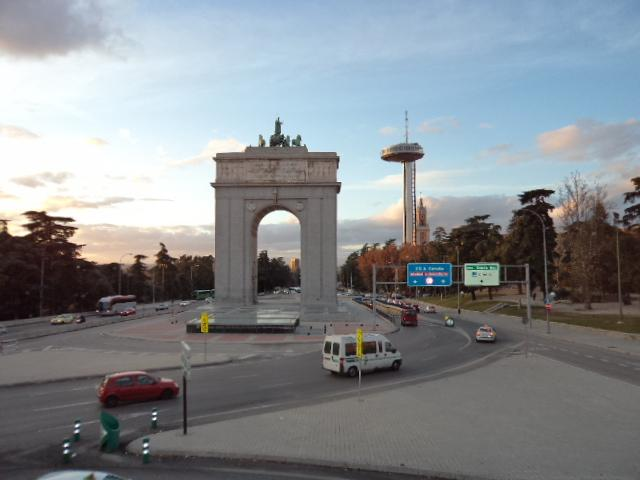
\includegraphics[scale=0.5]{Images/DSC00461}}
\end{userstory}

% Imprimir Prefactura
\begin{userstory}[tb:prueba]
	\storyname{Imprimir Prefactura}
	\storyuser{Legalizador}
	\storyiter{4}
	\storypriority{Alta}
	\storyrisk{Media}
	\storypoints{2}
	\storyprogrammer{Técn. Carlos Brayan Rámila Chorens}
	\storydescription{
		Permite al usuario poder acceder a la opción de imprimir la prefactura.
	}	
	\storyobservation{
	}
	%\storyinterface{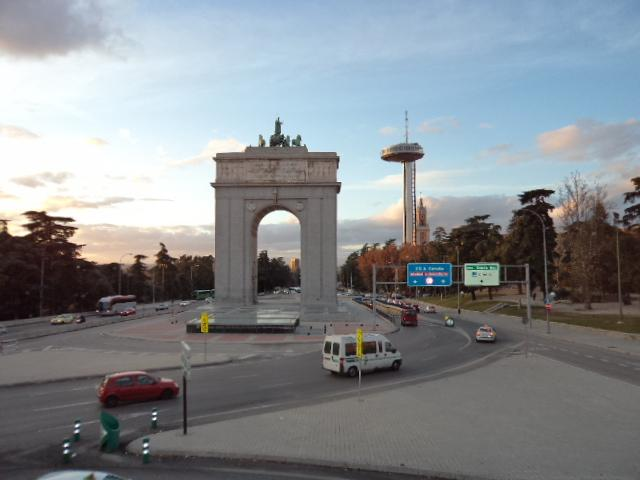
\includegraphics[scale=0.5]{Images/DSC00461}}
\end{userstory}

% Solicitar Cita al notario
\begin{userstory}[tb:prueba]
	\storyname{Solicitar Cita al notario}
	\storyuser{Cliente}
	\storyiter{4}
	\storypriority{Alta}
	\storyrisk{Media}
	\storypoints{2}
	\storyprogrammer{Técn. Carlos Brayan Rámila Chorens}
	\storydescription{
		Permite al usuario poder acceder a la opción de solicitar una cita, donde se muestra una página con un formulario a rellenar con los siguientes campos:
		
		\begin{itemize}
			\item Nombre
			\item Apellidos
			\item Dirección Particular
			\item Ci
			\item Teléfono de localización 
			\item Motivo por el cual Solicita la cita
		\end{itemize}
		
	}	
	\storyobservation{
	}
	%\storyinterface{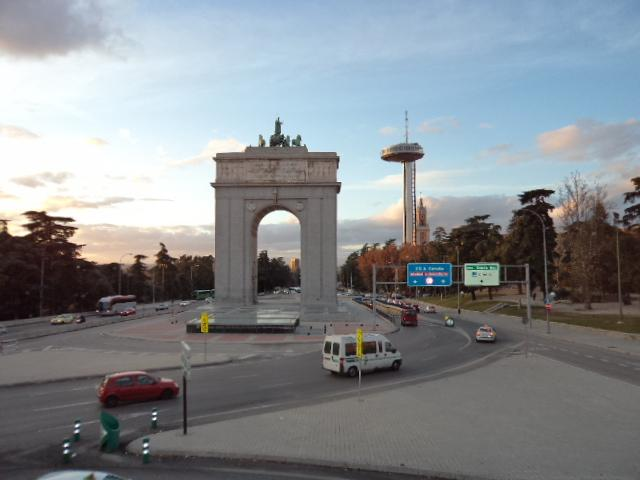
\includegraphics[scale=0.5]{Images/DSC00461}}
\end{userstory}

% Aceptar Cita
\begin{userstory}[tb:prueba]
	\storyname{Aceptar Cita}
	\storyuser{Notario}
	\storyiter{1.5}
	\storypriority{Alta}
	\storyrisk{Media}
	\storypoints{2}
	\storyprogrammer{Técn. Carlos Brayan Rámila Chorens}
	\storydescription{
			Permite al usuario poder acceder a la opción de Aceptar Cita, donde se muestra una página con un mensaje de advertencia.
			Estas seguro
			¡Esta acción sera notificada al cliente!
	}
	\storyobservation{
	}	
	%\storyinterface{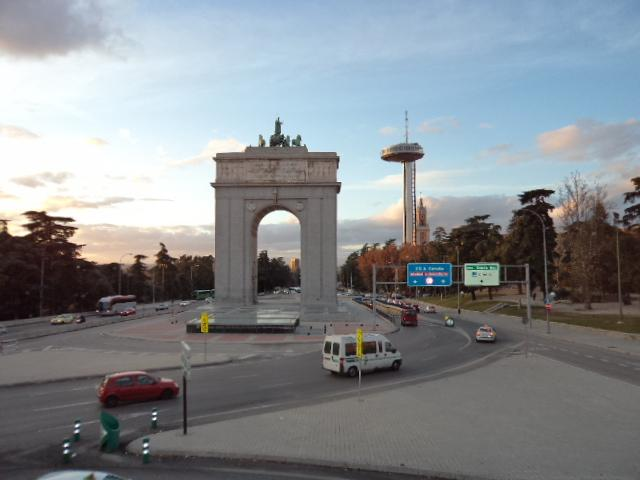
\includegraphics[scale=0.5]{Images/DSC00461}}
\end{userstory}




